% ============================================================
%  SimpleRNN vs LSTM Forecasting Notebook — Conceptual Description
%  Compile with: pdflatex (twice) or lualatex
%  Required packages: tikz, pgf, geometry, booktabs, array,
%                     tabularx, adjustbox, hyperref, microtype, parskip
% ============================================================
\documentclass[11pt, a4paper]{article}

% ── Packages ────────────────────────────────────────────────
\usepackage[T1]{fontenc}
\usepackage[utf8]{inputenc}
\usepackage[margin=2.4cm, top=2.8cm, bottom=2.8cm]{geometry}
\usepackage[expansion=false]{microtype}
\usepackage{parskip}
\usepackage{amsmath}
\usepackage{booktabs}
\usepackage{array}
\usepackage{tabularx}
\usepackage{adjustbox}
\usepackage{hyperref}
\usepackage{xcolor}
\usepackage{enumitem}
% To make labels Sans-Serif and Bold
\setlist[description]{font=\rmfamily\slshape}

% ── TikZ ────────────────────────────────────────────────────
\usepackage{tikz}
\usetikzlibrary{
  shapes.geometric,
  arrows.meta,
  positioning,
  fit,
  backgrounds,
  calc
}

\usetikzlibrary{shapes.geometric, arrows.meta, positioning, fit, backgrounds, calc}

% ── Colour definitions (matching SVG palette) ────────────────
\definecolor{grayFill}{HTML}{D3D1C7}
\definecolor{grayStroke}{HTML}{888780}
\definecolor{grayTxt}{HTML}{2C2C2A}
\definecolor{axisFill}{HTML}{F1EFE8}
\definecolor{axisTxt}{HTML}{5F5E5A}
\definecolor{tealFill}{HTML}{9FE1CB}
\definecolor{tealStroke}{HTML}{0F6E56}
\definecolor{tealTxt}{HTML}{04342C}
\definecolor{purpleFill}{HTML}{CECBF6}
\definecolor{purpleStroke}{HTML}{534AB7}
\definecolor{purpleTxt}{HTML}{26215C}
\definecolor{coralFill}{HTML}{F5C4B3}
\definecolor{coralStroke}{HTML}{993C1D}
\definecolor{coralTxt}{HTML}{4A1B0C}
\definecolor{dashColor}{HTML}{B4B2A9}

% ── Node styles ─────────────────────────────────────────────
\tikzset{
	base/.style={
		rectangle, rounded corners=5pt,
		text width=4.0cm, align=center,
		minimum height=1.1cm,
		inner sep=6pt,
		draw, line width=0.4pt,
		font=\small
	},
	% structural / entry nodes
	gray node/.style={base,
		fill=grayFill, draw=grayStroke, text=grayTxt},
	% axis banner (dashed)
	axis node/.style={base,
		fill=axisFill, draw=dashColor,
		text=axisTxt, dashed,
		text width=12.8cm, minimum height=0.9cm},
	% teal — Axis A
	teal node/.style={base,
		fill=tealFill, draw=tealStroke, text=tealTxt},
	% purple — Axis B
	purple node/.style={base,
		fill=purpleFill, draw=purpleStroke, text=purpleTxt},
	% coral — Axis C
	coral node/.style={base,
		fill=coralFill, draw=coralStroke, text=coralTxt},
	% narrow coral for Transformer box
	coral narrow/.style={coral node, text width=1.6cm},
	% arrow style
	arr/.style={-{Stealth[length=5pt,width=4pt]},
		line width=0.6pt, color=grayStroke},
	% axis label above arrows
	axlbl/.style={font=\scriptsize, text=axisTxt}
}

% ── Colour palette ──────────────────────────────────────────
\definecolor{clrGray}{HTML}{D3D1C7}
\definecolor{clrPurple}{HTML}{CECBF6}
\definecolor{clrTeal}{HTML}{9FE1CB}
\definecolor{clrGreen}{HTML}{C0DD97}
\definecolor{clrAmber}{HTML}{FAC775}
\definecolor{clrPurpleTxt}{HTML}{26215C}
\definecolor{clrTealTxt}{HTML}{04342C}
\definecolor{clrGreenTxt}{HTML}{173404}
\definecolor{clrAmberTxt}{HTML}{412402}
\definecolor{clrGrayTxt}{HTML}{2C2C2A}
\definecolor{clrBorder}{HTML}{888780}
\definecolor{clrDash}{HTML}{B4B2A9}

% ── TikZ node styles ────────────────────────────────────────
\tikzset{
	base/.style={
		rectangle, rounded corners=4pt, align=center,
		inner sep=4pt, draw, line width=0.4pt
	},
	gray nd/.style={base, minimum width=162mm, minimum height=11mm,
		fill=grayFill,   draw=grayStroke,   text=grayTxt,
		font=\fontsize{7.5}{9.5}\selectfont},
	axis nd/.style={base, minimum width=162mm, minimum height=9mm,
		fill=axisFill,   draw=dashColor,    text=axisTxt, dashed,
		font=\fontsize{7}{9}\selectfont},
	teal nd/.style={base, minimum width=48mm,  minimum height=13mm,
		fill=tealFill,   draw=tealStroke,   text=tealTxt,
		font=\fontsize{7}{9}\selectfont},
	purp nd/.style={base, minimum width=48mm,  minimum height=13mm,
		fill=purpleFill, draw=purpleStroke, text=purpleTxt,
		font=\fontsize{7}{9}\selectfont},
	purp sm/.style={base, minimum width=27mm,  minimum height=16mm,
		fill=purpleFill, draw=purpleStroke, text=purpleTxt,
		font=\fontsize{7}{9}\selectfont},
	cora nd/.style={base, minimum width=48mm,  minimum height=13mm,
		fill=coralFill,  draw=coralStroke,  text=coralTxt,
		font=\fontsize{7}{9}\selectfont},
	cora wd/.style={base, minimum width=37mm,  minimum height=16mm,
		fill=coralFill,  draw=coralStroke,  text=coralTxt,
		font=\fontsize{7}{9}\selectfont},
	cora nm/.style={base, minimum width=16mm,  minimum height=16mm,
		fill=coralFill,  draw=coralStroke,  text=coralTxt,
		font=\fontsize{7}{9}\selectfont},
	arr/.style={-{Stealth[length=4pt,width=3pt]},
		line width=0.5pt, color=grayStroke},
	albl/.style={font=\fontsize{6}{7.5}\selectfont, text=axisTxt}
}

\usepackage{forest}
\forestset{
	mono tree/.style={
		for tree={
			font=\sffamily,
			align=center,
			text width=5.2cm,
			minimum height=1.1cm,
			rounded corners=2pt,
			draw=black,
			thick,
			fill=white,
			edge={black, thick},
			l sep=10mm,
			s sep=5mm,
			anchor=center,
		},
		where level=0{
			font=\sffamily\bfseries\large,
			text width=6.5cm,
			minimum height=1.4cm,
			rounded corners=4pt,
			line width=1.2pt,
			draw=black,
		}{},
		where level=1{
			font=\sffamily\normalsize,
			line width=0.6pt,
			draw=black!80,
			edge={black!70, thick},
		}{},
	}
}

% ── Helpers ─────────────────────────────────────────────────
\newcommand{\sub}[1]{\\[2pt]{\footnotesize\normalfont #1}}
\newcolumntype{Y}{>{\raggedright\arraybackslash}X}

% ============================================================
\begin{document}

\section*{Notebook Construction and Audit Strategies}

This section outlines two complementary frameworks for working with
computational notebooks in machine learning and data science contexts:
a \textbf{Construction Framework} for authoring new notebooks, and an
\textbf{Audit Framework} for reviewing existing ones. Keeping these
separate prevents the common mistake of evaluating while still
constructing, which leads to incomplete analysis of both.

The two frameworks operate within a feedback loop, illustrated in
Figure~\ref{fig:notebook-lifecycle}.

%-----------------------------------------------------------------------
% FIGURE: Notebook Development Lifecycle
%-----------------------------------------------------------------------
\begin{figure}[ht]
	\centering
	
	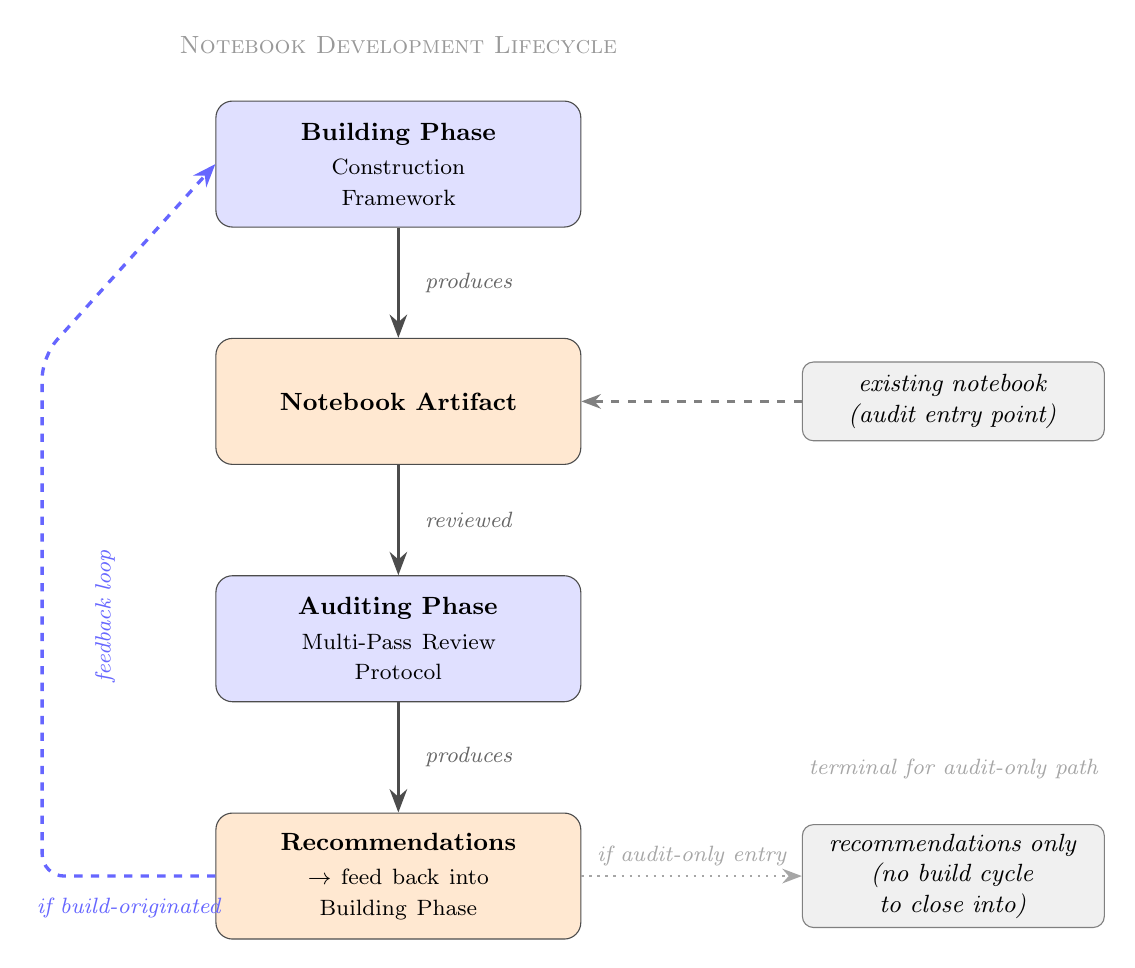
\begin{tikzpicture}[
		%--- Node Styles ---------------------------------------------------
		phase/.style={
			rectangle,
			rounded corners=6pt,
			draw=black!70,
			fill=blue!12,
			text width=44mm,
			minimum height=16mm,
			align=center,
			font=\bfseries\small
		},
		artifact/.style={
			rectangle,
			rounded corners=6pt,
			draw=black!70,
			fill=orange!18,
			text width=44mm,
			minimum height=16mm,
			align=center,
			font=\bfseries\small
		},
		entry/.style={
			rectangle,
			rounded corners=4pt,
			draw=black!50,
			fill=gray!12,
			text width=36mm,
			minimum height=10mm,
			align=center,
			font=\small\itshape
		},
		%--- Arrow Styles --------------------------------------------------
		mainarrow/.style={
			->,
			>=Stealth,
			line width=1.2pt,
			draw=black!70
		},
		entryarrow/.style={
			->,
			>=Stealth,
			line width=0.9pt,
			draw=black!50,
			dashed
		},
		feedbackarrow/.style={
			->,
			>=Stealth,
			line width=1.2pt,
			draw=blue!60,
			dashed,
			rounded corners=8pt
		},
		terminalarrow/.style={
			->,
			>=Stealth,
			line width=0.9pt,
			draw=gray!70,
			dotted
		},
		%--- Label Style ---------------------------------------------------
		edgelabel/.style={
			font=\footnotesize\itshape,
			text=black!60,
			midway,
			right=2mm
		}
		]
		
		%--- Main Column Nodes (top to bottom) ---------------------------------
		
		\node[phase] (build)
		{\textsc{Building Phase}\\[3pt]
			\normalfont\footnotesize Construction\\Framework};
		
		\node[artifact, below=14mm of build] (artifact)
		{\textsc{Notebook Artifact}};
		
		\node[phase, below=14mm of artifact] (audit)
		{\textsc{Auditing Phase}\\[3pt]
			\normalfont\footnotesize Multi-Pass Review\\Protocol};
		
		\node[artifact, below=14mm of audit] (reco)
		{\textsc{Recommendations}\\[3pt]
			\normalfont\footnotesize $\rightarrow$ feed back into\\Building Phase};
		
		%--- Entry Point Node (existing notebook) ------------------------------
		
		\node[entry, right=28mm of artifact] (existing)
		{existing notebook\\(audit entry point)};
		
		\node[entry, right=28mm of reco] (terminal)
		{recommendations only\\(no build cycle to close into)};
		
		%--- Main Flow Arrows --------------------------------------------------
		
		\draw[mainarrow] (build)    -- node[edgelabel]{produces} (artifact);
		\draw[mainarrow] (artifact) -- node[edgelabel]{reviewed} (audit);
		\draw[mainarrow] (audit)    -- node[edgelabel]{produces} (reco);
		
		%--- Dashed Entry Arrow ------------------------------------------------
		
		\draw[entryarrow] (existing.west) -- (artifact.east);
		
		%--- Terminal Path for Audit-Only Entries -------------------------------
		% Shows that recommendations from an audit-only entry do not
		% automatically close the loop back into Building Phase.
		%
		% NOTE: the feedback arrow (reco -> build) and the terminal arrow
		% (reco -> terminal) are mutually exclusive outcomes, conditioned
		% on entry path -- not simultaneous edges out of the same reco
		% instance. Rendered here as alternate branches labeled by
		% originating path, not as two live edges from one node.
		
		\draw[terminalarrow] (reco.east) -- (terminal.west)
		node[midway, above, font=\footnotesize\itshape, text=gray!70]
		{if audit-only entry};
		
		%--- Feedback Loop Arrow -----------------------------------------------
		% Runs up the left side from Recommendations back to Building Phase
		
		\draw[feedbackarrow]
		(reco.west)
		-- ++(-22mm, 0)
		-- ++(0,  66mm)
		-- (build.west);
		
		\node[font=\footnotesize\itshape, text=blue!60]
		at ($(reco.west) + (-11mm, -4mm)$)
		{if build-originated};
		
		%--- Feedback Loop Label -----------------------------------------------
		
		\node[font=\footnotesize\itshape, text=blue!60, rotate=90]
		at ($(reco.west) + (-14mm, 33mm)$)
		{feedback loop};
		
		\node[font=\footnotesize\itshape, text=gray!70]
		at ($(terminal.north) + (0, 7mm)$)
		{terminal for audit-only path};
		
		%--- Diagram Title Label -----------------------------------------------
		
		\node[font=\small\scshape, text=black!40]
		at ($(build.north) + (0, 7mm)$)
		{Notebook Development Lifecycle};
		
	\end{tikzpicture}
	
	\caption{%
	The Notebook Development Lifecycle. The \textbf{Construction Framework}
	(Part~I) produces a notebook artifact, assessed by the
	\textbf{Audit Framework} (Part~II) via a six-pass review protocol.
	For notebooks that originate in the Building Phase, the resulting
	recommendations feed back into a revised construction cycle, forming
	a closed feedback loop. An existing notebook (dashed entry) may
	instead enter the lifecycle directly at the artifact stage for
	audit-only workflows; in that case recommendations are a terminal
	deliverable rather than a loop closure, unless the notebook is
	subsequently routed into the Building Phase.
	}
	\label{fig:notebook-lifecycle}
\end{figure}

%-----------------------------------------------------------------------
\subsection*{Part I — Notebook Construction Framework}
%-----------------------------------------------------------------------

The Construction Framework is a \textit{forward-looking prescription}:
it guides the notebook author in producing a well-structured, reproducible,
and maintainable artifact from the ground up. It is organized into three
sequential phases.

% ── Diagram: Construction Strategy Tree ───────────────────────────────
\begin{figure}[ht]
	\centering
	\resizebox{\textwidth}{!}{%
		\begin{forest}
			mono tree,
			[Notebook Construction\\Strategy
			[Modular\\Section Design]
			[{Reproducibility Standards\\(seeds, environments)}]
			[Narrative Documentation\\Guidelines]
			[Output Artifact\\Management]
			]
		\end{forest}
	}
	\caption{High-level pillars of the Notebook Construction Framework.}
	\label{fig:construction-tree}
\end{figure}

\vspace{0.5cm}

\begin{description}
	
	\item[Phase 1 — Scaffold:]
	Establish the structural and reproducibility foundation before writing
	any logic:
	\begin{itemize}
		\item Define the notebook's \textbf{single responsibility} —
		one notebook should correspond to one coherent workflow
		or experiment.
		\item Create standard section headers as markdown cells, following
		this canonical order:
		\begin{enumerate}
			\item Environment \& Dependencies
			\item Configuration \& Global Parameters
			\item Data Ingestion
			\item Preprocessing \& Feature Engineering
			\item Model Definition \& Training
			\item Evaluation \& Metrics
			\item Artifact Export (models, plots, reports)
			\item Conclusions \& Next Steps
		\end{enumerate}
		\item Pin the execution environment upfront via
		\texttt{requirements.txt}, \texttt{conda.yaml},
		or \texttt{pyproject.toml}.
		\item Set global reproducibility controls: random seeds,
		deterministic flags, and device configuration.
	\end{itemize}
	
	\item[Phase 2 — Write:]
	Author each section incrementally, following these discipline rules:
	\begin{itemize}
		\item Work through \textbf{one section at a time}
		(Divide and Conquer principle).
		\item Accompany every code cell with a markdown explanation
		of intent and expected output.
		\item Avoid burying logic inside loops or helper calls
		without commentary.
		\item Prefer \textbf{explicit variable passing} over hidden
		or global state to maintain cell independence.
		\item Summarize repetitive code patterns with a general
		description and highlight any meaningful variations;
		three or more similar blocks should be treated as a
		refactoring candidate.
		\item Route all persisted outputs (models, plots, reports)
		through a single, versioned export convention defined at
		the start of the section — never write artifacts ad hoc
		from arbitrary cells.
	\end{itemize}
	
	\item[Phase 3 — Validate During Writing:]
	Continuously verify correctness as each section is completed:
	\begin{itemize}
		\item Restart the kernel and run all cells after completing
		each section.
		\item Confirm \textbf{cell idempotency}: every cell should
		produce the same result when re-executed independently.
		\item Verify that outputs match expectations before proceeding
		to the next section.
		\item Ensure cell execution order is strictly linear
		and free of hidden dependencies.
		\item Confirm that exported artifacts land in the designated
		output location with the expected naming and versioning
		convention before moving to the next section.
	\end{itemize}
	
\end{description}

%-----------------------------------------------------------------------
\subsection*{Part II — Notebook Audit Framework}
%-----------------------------------------------------------------------

The Audit Framework is a \textit{backward-looking diagnostic}: it guides
a reviewer, collaborator, or AI assistant in systematically assessing the
quality, correctness, and risk profile of an existing notebook.

To execute this efficiently, the reviewer should employ guiding tactics
such as dividing the notebook into logical modules, prioritizing critical
ML pipeline blocks over repetitive exploration cells, using hierarchical
descriptions (high-level summaries first, drill-downs later), and
summarizing repetitive code patterns rather than analyzing each
individually. When a human collaborator specifies focus areas in advance
(e.g., "check only for data leakage" or "skip code style"), the reviewer
should scope the six-pass review protocol to those areas rather than
executing all six passes uniformly.

The framework is formalized as a six-pass review protocol, applied
sequentially. Any pass included in scope is executed in full, following
its own deliverable requirements below.

Where a pass deliverable is a score, the reviewer rates on a three-level
scale — \textit{Low Risk}, \textit{Moderate Risk}, \textit{High Risk} —
based on the number and severity of unresolved items identified within
that pass, rather than a numeric or percentage scale.

% ── Diagram: Audit Strategy Tree ──────────────────────────────────────
\begin{figure}[ht]
	\centering
	\resizebox{\textwidth}{!}{%
		\begin{forest}
			mono tree,
			[Notebook Audit\\Strategy
			[{Multi-Pass Incremental\\Analysis}]
			[Hierarchical\\Review Depth]
			[Pattern Summarization\\with Thresholds]
			[{User-Guided Focus Areas\\(AI-assisted context)}]
			]
		\end{forest}
	}
	\caption{High-level pillars of the Notebook Audit Framework.}
	\label{fig:audit-tree}
\end{figure}

\begin{description}
	
	\item[Pass 1 — Structural Overview:]
	Establish a high-level map of the notebook before examining any logic:
	\begin{itemize}
		\item Record any user-specified focus areas or exclusions
		that will scope the remaining five passes.
		\item Assess whether the notebook has clear, navigable
		section headers.
		\item Confirm that the notebook has a single, coherent purpose.
		\item Verify that cell execution order is linear and safe.
		\item Identify any immediately visible red flags
		(e.g., missing outputs, broken imports, orphaned cells).
		\item \textit{Deliverable:} Section map, preliminary red flags
		list, and recorded focus-area scope (if specified).
	\end{itemize}
	
	\item[Pass 2 — Reproducibility Check:]
	Assess whether the notebook can be reliably re-executed:
	\begin{itemize}
		\item Verify that dependencies are declared and version-pinned.
		\item Confirm that random seeds are set globally and consistently.
		\item Flag any hardcoded file paths, credentials, or
		environment-specific assumptions.
		\item Determine whether the notebook can run end-to-end
		on a fresh kernel without manual intervention.
		\item \textit{Deliverable:} Reproducibility risk score
		(Low / Moderate / High).
	\end{itemize}
	
	\item[Pass 3 — Data Integrity Review:]
	Examine the data pipeline for correctness and leakage risks:
	\begin{itemize}
		\item Confirm that the train/test split is performed
		\textbf{before} any preprocessing step.
		\item Identify signs of \textbf{data leakage}
		(e.g., scaling fitted on the full dataset).
		\item Verify that missing data is handled consistently
		across splits.
		\item Check that data types, shapes, and distributions
		are validated at ingestion.
		\item \textit{Deliverable:} Data pipeline integrity report.
	\end{itemize}
	
	\item[Pass 4 — ML Correctness Audit:]
	Evaluate the soundness of the machine learning methodology:
	\begin{itemize}
		\item Confirm that the evaluation metric is appropriate
		for the task and class distribution.
		\item Verify that cross-validation is applied correctly
		and without leakage.
		\item Ensure hyperparameter tuning is performed on
		validation data only, never on test data.
		\item Check that model performance is contextualized
		against a meaningful baseline.
		\item \textit{Deliverable:} ML correctness checklist.
	\end{itemize}
	
	\item[Pass 5 — Code Quality Review:]
	Assess the maintainability and clarity of the code:
	\begin{itemize}
		\item Flag repetitive code blocks that exceed the
		three-block threshold as refactoring candidates.
		\item Identify dead code, unused imports, and
		redundant variable assignments.
		\item Assess whether variable and function names
		are meaningful and consistent.
		\item Check for bloated cell outputs
		(e.g., printing entire dataframes or raw tensors).
		\item \textit{Deliverable:} Code quality and smell report.
	\end{itemize}
	
	\item[Pass 6 — Deployment Readiness:]
	Determine whether the notebook is suitable for production or
	publication:
	\begin{itemize}
		\item Verify that model artifacts are explicitly saved
		with versioned filenames.
		\item Confirm that inference logic is separable from
		training logic.
		\item Check that compute and memory constraints are
		documented or profiled.
		\item Ensure a complete environment export is present
		and up to date.
		\item Flag any data privacy or PII handling concerns.
		\item \textit{Deliverable:} Deployment readiness score
		(Low / Moderate / High).
	\end{itemize}
	
\end{description}

%-----------------------------------------------------------------------
\subsection*{Applying the Two Frameworks}
%-----------------------------------------------------------------------

The appropriate framework depends on the context of engagement
with the notebook:

\begin{description}
	
	\item[Use the Construction Framework when:]
	starting a new notebook or experiment; restructuring a disorganized
	notebook by discarding its existing structure and rebuilding section
	organization from scratch; or creating a reusable notebook template
	for a team or project.
	
	\item[Use the Audit Framework when:]
	reviewing a collaborator's notebook; preparing a notebook for
	production deployment or academic publication; conducting a
	pre-merge or pre-deployment review; or using an AI assistant
	to analyze submitted notebook code.
	
	\item[Use Both Frameworks iteratively when:]
	authoring and self-reviewing during active development;
	collaborating or pair-programming in real time; or refactoring
	an existing notebook into a cleaner, production-ready version while
	preserving its existing section structure and logic.
	
\end{description}

\noindent
The Construction Framework and Audit Framework complement each other
within a feedback loop: the construction phase produces a notebook
artifact, the audit phase diagnoses its weaknesses, and the resulting
recommendations feed back into a revised construction cycle. This
closure applies to notebooks that begin in the Building Phase; for
notebooks entering via the audit-only path, the loop remains open
unless the notebook is subsequently taken up for construction, as
illustrated in Figure~\ref{fig:notebook-lifecycle}.

\subsection*{Prompt Crafting}

For implementing an LLM prompt engineering framework, the following prompt-draft iterations are presented in increasing order of complexity:
\begin{description}
	\item[Lap 1. Coarse evaluation]\;  
	
\vspace{.3cm}
\rule{\textwidth}{0.3pt}

{\small\sffamily
TASK: Analyze the provided Jupyter Notebook and produce a structured audit. Proceed to systematically analyze the codebase, examining each section dependently. After all reports have been generated, compare them without looking at the code. 
once you have a comparison, compare the mission report to the code base and point out any discrepancies

PHASE 1 — DOCUMENTATION
[Section 1: Overall Purpose — 2-3 sentences]
[Section 2: Code Block Descriptions — numbered by executable cells only, 
with merged categories: Logic and Flow, Data and State, 
Operations and Methods, Side Effects]
[section 3: Pseudocode any functions that seem too complicated for the naked eye. Revise all comments. Suggest a new code naming convention.]
[Section 4: Pipeline Summary — 3-5 sentences if dependencies exist]

PHASE 2 — CRITICAL AUDIT
[Evaluate and score the ORIGINAL CODE (not your descriptions) for:
- Cross-block consistency in data types and variable naming
- Redundant computation or unnecessary I/O
- Contradictory logic or unreachable branches
- Missing error handling or validation]

Suggest a Gate decision	

add fingerprint "lap 0" and timestamp
}

\rule{\textwidth}{0.3pt}

\vspace{.3cm}
	\item[Lap 2. More  refined evaluation]\;  

\vspace{.3cm}
\rule{\textwidth}{0.3pt}

{\small\sffamily
Task: Analyze the provided Jupyter Notebook code and extract the following structured information. Number code blocks sequentially (Block 1, Block 2, etc.) based on top-to-bottom visual appearance, strictly ignoring Jupyter's native execution counters (e.g., [ ]).
	
	1 - Overall Purpose / Goal
	Provide a clear and concise summary (2-3 sentences maximum) of the notebook’s main objective, including:
	
	- The problem it solves
	- The type of input it expects
	- The output or result it produces
	2 - Conceptual Description of Each Code Block
	Apply the following rules for processing cells:
	
	Consolidation: Group all library imports, package installations (e.g., !pip), and magic commands (e.g., %%time) into a single first block titled "Environment Setup".
	Filtering: Skip and do not include pure markdown cells, raw text cells, empty cells, or cells that throw execution errors in the block list below.
	For all remaining valid executable code blocks, extract:
	
	Logic Flow: Step-by-step reasoning behind the code's execution.
	Data Transformations: What goes in (inputs) and what comes out (outputs) regarding data shapes/types (e.g., "Transforms DataFrame X from wide to long format").
	Model/Algorithm Operations: Any ML, statistical, or computational methods applied.
	Key Variables/Parameters: Important identifiers, hyperparameters, or configurations.
	Side Effects: File I/O, state changes, printed output, API calls, etc.
	3 - Output Format Requirements
	Structure your response exactly as follows, using the exact headings provided:
	
	1 - Overall Purpose / Goal
	[Your summary here]
	
	Code Block Descriptions
	Block 1 - Environment Setup
	Logic Flow: N/A
	Data Transformations: N/A
	Model/Algorithm Operations: N/A
	Key Variables/Parameters: [List imported libraries/versions if specified]
	Side Effects: [List any installations or magic command outputs]
	
	Block 2 - [Short Descriptive Title]
	Logic Flow: ...
	Data Transformations: ...
	Model/Algorithm Operations: ...
	Key Variables/Parameters: ...
	Side Effects: ...
	[Continue pattern for all blocks...]
	
	4 - Pipeline Summary
	Explain how the extracted blocks connect to form a complete pipeline:
	
	Trace the data flow from the first computational block to the last.
	Detail any branching, looping, or conditional paths across blocks.
	5 - Cross-Block Code Quality Audit
	Audit the notebook's underlying code for structural and logical issues. Address each of the following points strictly using bullet points:
	
	Coherence and Consistency: [Note any mismatches between data transformations and downstream usage]
	Redundancy and Waste: [Identify any inefficient repeated computation or redundant data transformations]
	Contradictory Logic: [Point out any instances where later blocks logically contradict or overwrite earlier blocks]
	If no issues are found in a category, write "None detected."
	
	add fingerprint "lap 1" and timestamp
	
}
\vspace{.3cm}
\rule{\textwidth}{0.3pt}

	\item[Lap 2. Structured evaluation]\;  
	A 3-level structure for engineering prompts is assumed that maps cleanly onto the existing six passes without requiring changes to the framework itself:
	
	\begin{enumerate}{ }
		\item  \textit{Level 1 — Conceptual} (Passes 1–2):
		Structural Overview + Reproducibility Check. Establishes whether the notebook is coherent and re-runnable at all, before any deep inspection is worth doing.
		
		\item \textit{Level 2 — Methodological} (Passes 3–4):
		Data Integrity Review + ML Correctness Audit. Addresses whether the pipeline and modeling logic are scientifically sound — the "does this work correctly" layer.
		
		\item \textit{Level 3 — Implementation]} (Passes 5–6):
		Code Quality Review + Deployment Readiness. Addresses how the working logic is written and packaged — the most granular, code-level layer.
	\end{enumerate}
\end{description}

\subsubsection*{Level 1 -- Conceptual Purpose} 
 determine whether the notebook is coherent and reliably re-executable before investing time in deeper review.

Step 1.1 — Scope the audit: 

Record any user-specified focus areas or exclusions (if a collaborator has scoped the review in advance).
Note this scope explicitly — it determines which of the remaining passes/levels get full attention later.

Step 1.2 — Map the structure

Assess whether the notebook has clear, navigable section headers.
Confirm the notebook has a single, coherent purpose (not multiple unrelated experiments bundled together).
Verify cell execution order is linear and free of hidden dependencies.

Step 1.3 — Scan for immediate red flags

Identify visible issues without deep inspection: missing outputs, broken imports, orphaned cells.

Step 1.4 — Check reproducibility inputs

Verify dependencies are declared and version-pinned (requirements.txt, conda.yaml, pyproject.toml, or equivalent).
Confirm random seeds are set globally and consistently.

Step 1.5 — Check reproducibility risks

Flag hardcoded file paths, credentials, or environment-specific assumptions.
Determine whether the notebook can run end-to-end on a fresh kernel without manual intervention.

Level 1 deliverables:

Section map,
Preliminary red flags list,
Recorded focus-area scope (if specified),
Reproducibility risk score (Low / Moderate / High)

Gate decision before moving to Level 2: if the notebook fails end-to-end execution or lacks a coherent single purpose, decide now whether to proceed to Level 2 anyway (methodological review can still surface findings) or to stop and flag Level 1 as blocking — the framework doesn't mandate either, so this is your call to make consistently across audits.

\vspace{.3cm}
\rule{\textwidth}{0.3pt}

{\small\sffamily

You are performing a Level 1 (Conceptual) audit of a Jupyter notebook.
This notebook is moderate length (approximately 400-600 lines) — read
it in full before reporting; do not sample or skim sections.

Your ONLY objective at this level is to determine whether the notebook
is structurally coherent and reliably re-executable. Do NOT evaluate
code quality, ML methodology, data leakage, or deployment readiness —
those belong to later audit levels and are out of scope here.

Follow these steps in order:

STEP 1 — SCOPE
- Note if I have specified any focus areas or exclusions for this audit.
If none given, assume full Level 1 scope.

STEP 2 — STRUCTURE MAP
- List the notebook's section headers (markdown cells) in order.
- State whether the notebook has a single, coherent purpose, or if it
bundles multiple unrelated workflows/experiments.
- Verify cell execution order is linear — flag any cell that appears to
depend on a later cell, or any out-of-order execution counts visible
in cell outputs.

STEP 3 — RED FLAGS SCAN
- Identify immediately visible issues: missing/empty outputs, broken or
unused imports, orphaned cells (code with no clear purpose or downstream
use), cells left in a non-executed state.

STEP 4 — REPRODUCIBILITY INPUTS
- Check whether dependencies are declared and version-pinned (look for
a requirements.txt, environment.yml, pyproject.toml, or an explicit
pip/conda install cell with pinned versions).
- Check whether random seeds are set globally (e.g., numpy, torch,
random, sklearn) and consistently applied before any stochastic
operation.

STEP 5 — REPRODUCIBILITY RISKS
- Flag hardcoded file paths, credentials, API keys, or any
environment-specific assumption (e.g., a path that only exists on
one machine).
- Assess whether the notebook could plausibly run end-to-end on a
fresh kernel without manual intervention. State your reasoning,
not just a yes/no.

OUTPUT FORMAT — return exactly these four items, nothing else:

1. Section map (ordered list of headers, or "no clear section headers"
if absent)
2. Preliminary red flags list (bullet points; write "none identified"
if empty)
3. Recorded focus-area scope (state "full scope" if none was specified)
4. Reproducibility risk score: Low / Moderate / High, with a
one-sentence justification tied to what you found in Steps 4-5

Do not add commentary, recommendations, or fixes at this stage —
Level 1 is diagnostic only. Do not comment on code style, variable
naming, or model correctness.

}

\rule{\textwidth}{0.3pt}

\vspace{.3cm}

\subsubsection*{Level 2 -- Methodological Purpose} 
determine whether the data pipeline and modeling methodology are scientifically sound, assuming Level 1 has already confirmed the notebook is structurally coherent and runnable.

Step 2.1 — Verify split ordering

Confirm that the train/test split is performed before any preprocessing step (scaling, encoding, imputation, feature engineering).

Step 2.2 — Check for pipeline-level leakage

Identify signs of data leakage introduced during preparation (e.g., a scaler, encoder, or imputer fitted on the full dataset rather than the training split alone).
Leakage introduced later, through cross-validation or model selection, is addressed in Step 2.5 — don't double-flag it here.

Step 2.3 — Check missing-data handling

Verify that missing data is handled consistently across the train and test splits (same strategy applied to both, fit only on training data).

Step 2.4 — Validate data at ingestion

Check that data types, shapes, and distributions are validated when the data is first loaded (not assumed silently downstream).

Step 2.5 — Verify cross-validation integrity

Confirm cross-validation folds preserve the train/test separation established in Step 2.1.
Check that no fold-selection, resampling, or preprocessing-within-CV step exposes validation or test data to the training process.

Step 2.6 — Check evaluation metric appropriateness

Confirm the evaluation metric fits the task and class distribution (e.g., accuracy on an imbalanced classification problem is a red flag).

Step 2.7 — Check hyperparameter tuning boundaries

Ensure hyperparameter tuning is performed on validation data only, never on the test set.

Step 2.8 — Check baseline comparison

Confirm model performance is contextualized against a meaningful baseline (e.g., a naive predictor, a simpler model, or a published benchmark) — not reported in isolation.

Level 2 deliverables:

Data pipeline integrity report (from Steps 2.1–2.4),
ML correctness checklist (from Steps 2.5–2.8)

Gate decision before moving to Level 3: if pipeline-level leakage is found in Step 2.2, decide whether downstream ML correctness findings (Steps 2.5–2.8) are still meaningful to report, since a leaky pipeline can invalidate reported model performance regardless of how sound the CV/tuning procedure is. As with the Level 1 gate, the framework doesn't mandate stopping — this is a call to make consistently across your audits.

\vspace{.3cm}
\rule{\textwidth}{0.3pt}

{\small\sffamily

You are performing a Level 2 (Methodological) audit of a Jupyter notebook.
This notebook is moderate length (approximately 400-600 lines) — read it
in full before reporting; do not sample or skim sections.

Assume Level 1 (structural/reproducibility review) has already been
completed. Your ONLY objective at this level is to determine whether the
data pipeline and modeling methodology are scientifically sound. Do NOT
comment on code style, variable naming, section headers, or deployment
readiness — those belong to other audit levels and are out of scope here.

Follow these steps in order:

STEP 1 — SPLIT ORDERING
- Locate where the train/test split occurs in the notebook.
- Confirm it happens BEFORE any preprocessing step (scaling, encoding,
imputation, feature engineering). If preprocessing precedes the split,
flag this explicitly and identify the exact cell(s) involved.

STEP 2 — PIPELINE-LEVEL LEAKAGE
- Identify any scaler, encoder, imputer, or feature-engineering step
fitted on the full dataset rather than the training split alone.
- Do NOT flag cross-validation or hyperparameter-tuning leakage here —
that belongs to Step 5.

STEP 3 — MISSING DATA HANDLING
- Verify missing data is handled with a strategy fit only on the
training data, then applied identically to the test data.
- Flag any case where the missing-data strategy is computed on the
full dataset or differs between splits.

STEP 4 — DATA VALIDATION AT INGESTION
- Check whether data types, shapes, and distributions are inspected or
validated when the data is first loaded (e.g., dtype checks, null
counts, shape assertions, distribution plots).
- Flag if the notebook proceeds directly to modeling without any
ingestion-time validation.

STEP 5 — CROSS-VALIDATION INTEGRITY
- Confirm cross-validation folds preserve the train/test separation
identified in Step 1.
- Check whether any fold-selection, resampling, or preprocessing step
inside the CV loop exposes validation or test data to training.

STEP 6 — EVALUATION METRIC APPROPRIATENESS
- Identify the evaluation metric(s) used.
- State whether the metric fits the task and class distribution (e.g.,
flag accuracy as a red flag on an imbalanced classification problem).

STEP 7 — HYPERPARAMETER TUNING BOUNDARIES
- Confirm hyperparameter tuning is performed only on validation data,
never on the test set. Identify the exact cell(s) where tuning occurs.

STEP 8 — BASELINE COMPARISON
- Check whether model performance is compared against a meaningful
baseline (naive predictor, simpler model, or published benchmark).
- Flag if performance is reported in isolation with no baseline context.

OUTPUT FORMAT — return exactly these two items, nothing else:

1. Data pipeline integrity report (Steps 1-4): for each step, state
PASS or FLAG, with the specific cell reference and a one-sentence
explanation for any flag.

2. ML correctness checklist (Steps 5-8): for each step, state PASS or
FLAG, with the specific cell reference and a one-sentence explanation
for any flag.

If pipeline-level leakage is found in Step 2, note this at the top of
your output as a blocking issue, since it can invalidate any performance
numbers evaluated in Steps 5-8 — but still complete and report Steps 5-8
regardless.

Do not propose fixes or rewrite code at this stage — Level 2 is
diagnostic only.

}

\rule{\textwidth}{0.3pt}

\vspace{.3cm}


\subsubsection*{Level 3 — Implementation
Purpose} 
determine whether the code is maintainable and clear, and whether the notebook is suitable for production or publication — assuming Level 1 has confirmed structural coherence and Level 2 has confirmed methodological soundness.
Step 3.1 — Flag repetitive code blocks

Identify code blocks that exceed the three-block threshold (three or more similar blocks) and mark them as refactoring candidates.

Step 3.2 — Identify dead code and unused elements

Flag unused imports, dead code paths, and redundant variable assignments.

Step 3.3 — Assess naming quality

Evaluate whether variable and function names are meaningful and used consistently throughout the notebook.

Step 3.4 — Check output hygiene

Flag bloated cell outputs (e.g., printing entire dataframes, raw tensors, or large arrays) that clutter the notebook without adding interpretive value.

Step 3.5 — Verify artifact export

Confirm model artifacts (models, plots, reports) are explicitly saved with versioned filenames, not left only in memory or overwritten without versioning.

Step 3.6 — Check inference/training separability

Confirm inference logic is separable from training logic — i.e., a saved model could be loaded and used for inference without re-running the training pipeline.

Step 3.7 — Check resource documentation

Verify that compute and memory constraints are documented or profiled (e.g., expected runtime, GPU/CPU requirements, peak memory usage).

Step 3.8 — Check environment completeness

Confirm a complete environment export is present and up to date (consistent with what Level 1 checked for reproducibility, but here verified for deployment sufficiency specifically).

Step 3.9 — Flag data privacy concerns

Identify any handling of PII or sensitive data without appropriate safeguards (anonymization, access control, exclusion from version control).

Level 3 deliverables:

Code quality and smell report (from Steps 3.1–3.4),
Deployment readiness score, Low / Moderate / High (from Steps 3.5–3.9)

\vspace{.3cm}
\rule{\textwidth}{0.3pt}

{\small\sffamily
You are performing a Level 3 (Implementation) audit of a Jupyter notebook.
This notebook is moderate length (approximately 400-600 lines) — read it
in full before reporting; do not sample or skim sections.

Assume Level 1 (structural/reproducibility review) and Level 2
(data pipeline/ML methodology review) have already been completed.
Your ONLY objective at this level is to assess code maintainability and
deployment readiness. Do NOT re-evaluate section structure, data leakage,
model correctness, or evaluation metrics — those belong to other audit
levels and are out of scope here.

Follow these steps in order:

STEP 1 — REPETITIVE CODE
- Identify any code pattern that repeats across three or more cells or
blocks (e.g., repeated plotting logic, repeated preprocessing steps
applied separately to each feature).
- Flag each as a refactoring candidate with the specific cell references.

STEP 2 — DEAD CODE AND UNUSED ELEMENTS
- Identify unused imports.
- Identify dead code paths (code that cannot be reached or has no
downstream effect).
- Identify redundant variable assignments (e.g., a variable reassigned
without ever being read in between).

STEP 3 — NAMING QUALITY
- Assess whether variable and function names are descriptive and
consistent throughout (e.g., not `df1`, `df2`, `tmp`, `x2` used
interchangeably with meaningful names elsewhere).
- Flag inconsistencies where the same concept is named differently in
different cells.

STEP 4 — OUTPUT HYGIENE
- Identify any cell output that prints an entire dataframe, raw tensor,
or large array without truncation, sampling, or summarization.
- Flag these as clutter that reduces notebook readability.

STEP 5 — ARTIFACT EXPORT
- Confirm that models, plots, and reports are explicitly saved to disk
with versioned or timestamped filenames.
- Flag any artifact that is generated but never saved, or saved with a
filename that would be overwritten on the next run.

STEP 6 — INFERENCE/TRAINING SEPARABILITY
- Determine whether a saved model could be loaded and used for
inference without re-running the training pipeline.
- Flag if inference logic is entangled with training logic in the same
cells with no clear separation point.

STEP 7 — RESOURCE DOCUMENTATION
- Check whether the notebook documents or profiles compute/memory
requirements (expected runtime, GPU/CPU needs, peak memory).
- Flag if no such documentation exists, especially for
computationally expensive cells (training loops, large matrix
operations).

STEP 8 — ENVIRONMENT COMPLETENESS
- Verify a complete, up-to-date environment export exists (e.g.,
requirements.txt, environment.yml) sufficient for someone else to
reproduce a deployment-ready environment — not just "the code runs,"
but "the exact dependency versions are captured."

STEP 9 — DATA PRIVACY CONCERNS
- Identify any handling of personally identifiable information (PII)
or sensitive data.
- Flag missing safeguards: no anonymization, no access control, data
or credentials committed directly into the notebook or version
control.

OUTPUT FORMAT — return exactly these two items, nothing else:

1. Code quality and smell report (Steps 1-4): for each step, list
findings with specific cell references; write "none identified" if
a step surfaces nothing.

2. Deployment readiness score: Low / Moderate / High (Steps 5-9), with
a bulleted justification — one bullet per step, stating PASS or
FLAG with a one-sentence reason for any flag.

If Step 8 findings overlap with a reproducibility check from Level 1,
note it briefly as "consistent with Level 1 finding" rather than
re-describing it in full — avoid duplicating that report.

Do not propose fixes or rewrite code at this stage — Level 3 is
diagnostic only.
}

\rule{\textwidth}{0.3pt}

\vspace{.3cm}


%\newpage
%\begin{tikzpicture}[
%	node distance=0.45cm and 1.0cm,
%	box/.style={
%		rectangle,
%		rounded corners,
%		draw,
%		align=center,
%		minimum width=3.4cm,
%		minimum height=0.8cm,
%		font=\small
%	},
%	arrow/.style={->, thick}
%	]
%	
%	\node[box] (A) {Goal: one-step Google\\Open price forecasting};
%	\node[box, below=of A] (B) {Load CSV from URL\\or local cache};
%	\node[box, below=of B] (C) {Validate columns:\\Open, High, Low, Close};
%	\node[box, below=of C] (D) {Clean numeric values\\and sort by Date};
%	\node[box, below=of D] (E) {Select target series:\\Open price};
%	\node[box, below=of E] (F) {Set config:\\TS, SPLIT, EP, H, LR};
%	
%	\node[box, below left=of F] (G) {Chronological\\train/test split};
%	\node[box, below=of G] (H) {Fit scaler\\on train only};
%	\node[box, below=of H] (I) {Create sliding windows};
%	
%	\node[box, below=of I] (J) {Define from-scratch\\SimpleRNN};
%	\node[box, below=of J] (K) {Tiny gradient check\\debug model only};
%	\node[box, below=of K] (L) {Train level-price\\RNN baseline};
%	
%	\node[box, below right=of F] (M) {Create differenced target:\\daily price change};
%	\node[box, below=of M] (N) {Train differenced RNN};
%	\node[box, below=of N] (O) {Train differenced\\RNN ensemble};
%	\node[box, below=of O] (P) {Train larger capacity\\RNN: H=128};
%	
%	\node[box, right=of F] (Q) {Naive persistence:\\tomorrow = today};
%	
%	% Merge point placed below both trained branches
%	\coordinate (merge) at ($(L.south)!0.5!(P.south) + (0,-1.0cm)$);
%	
%	\node[box, below=0.2cm of merge] (R) {One-step walk-forward\\predictions};
%	\node[box, below=of R] (S) {Evaluate RMSE\\and MAE};
%	\node[box, below=of S] (T) {Plot actual\\vs forecasts};
%	\node[box, below=of T] (U) {Compare against\\persistence baseline};
%	\node[box, below=of U] (V) {Interpret result:\\differencing helps RNN,\\persistence is hard to beat};
%	\node[box, below=of V] (W) {Inspect one prediction\\step by step};
%	\node[box, below=of W] (X) {Show inputs, hidden states,\\and final output};
%	
%	\draw[arrow] (A) -- (B);
%	\draw[arrow] (B) -- (C);
%	\draw[arrow] (C) -- (D);
%	\draw[arrow] (D) -- (E);
%	\draw[arrow] (E) -- (F);
%	
%	\draw[arrow] (F) -- (G);
%	\draw[arrow] (G) -- (H);
%	\draw[arrow] (H) -- (I);
%	\draw[arrow] (I) -- (J);
%	\draw[arrow] (J) -- (K);
%	\draw[arrow] (K) -- (L);
%	
%	\draw[arrow] (F) -- (M);
%	\draw[arrow] (M) -- (N);
%	\draw[arrow] (N) -- (O);
%	\draw[arrow] (O) -- (P);
%	
%	\draw[arrow] (F) -- (Q);
%	
%	% Route all forecast sources into the common prediction node
%	\draw[arrow] (L.south) |- (R.west);
%	\draw[arrow] (N.south) |- (R.east);
%	\draw[arrow] (O.south) |- (R.east);
%	\draw[arrow] (P.south) |- (R.east);
%	\draw[arrow] (Q.south) |- (R.east);
%	
%	\draw[arrow] (R) -- (S);
%	\draw[arrow] (S) -- (T);
%	\draw[arrow] (T) -- (U);
%	\draw[arrow] (U) -- (V);
%	\draw[arrow] (V) -- (W);
%	\draw[arrow] (W) -- (X);
%	
%\end{tikzpicture}
%
%SimpleRNN – single tanh activation, no gates (struggles with long-term dependencies).
%
%GRU – introduces reset and update gates (less complex than LSTM, fewer parameters).
%
%LSTM – introduces three gates (input, forget, output) + a separate cell state, making it the most expressive pure recurrent cell.
%%\newpage
%%\begin{tikzpicture}[
%%	node distance=1cm and 1.3cm,
%%	box/.style={
%%		rectangle,
%%		rounded corners,
%%		draw,
%%		align=center,
%%		minimum width=3cm,
%%		minimum height=0.8cm,
%%		font=\small
%%	},
%%	arrow/.style={->, thick}
%%	]
%%	
%%	\node[box] (A) {Past window\\of prices};
%%	\node[box, right=of A] (B) {RNN hidden\\state};
%%	\node[box, right=of B] (C) {One-step\\forecast};
%%	\node[box, right=of C] (D) {Compare with\\actual next price};
%%	
%%	\node[box, below=1.4cm of A] (E) {Past price\\changes};
%%	\node[box, right=of E] (F) {RNN predicts\\next change};
%%	\node[box, right=of F] (G) {Yesterday's real price\\+ predicted change};
%%	
%%	\draw[arrow] (A) -- (B);
%%	\draw[arrow] (B) -- (C);
%%	\draw[arrow] (C) -- (D);
%%	
%%	\draw[arrow] (E) -- (F);
%%	\draw[arrow] (F) -- (G);
%%	\draw[arrow] (G) -- (D);
%%	
%%\end{tikzpicture}
%
%
%\begin{tikzpicture}[
%	node distance=0.9cm and 1.4cm,
%	box/.style={
%		rectangle,
%		rounded corners,
%		draw,
%		align=center,
%		text width=3.7cm,
%		minimum height=0.85cm,
%		font=\small
%	},
%	bluebox/.style={
%		box,
%		fill=blue!12,
%		draw=blue!70!black,
%		line width=1.1pt,
%		text=black
%	},
%	arrow/.style={->, thick}
%	]
%	
%	\node[box] (A) {Goal: one-step forecast\\of Google Open price};
%	\node[box, below=of A] (B) {Load data\\and preprocessing};
%	\node[box, below=of B] (H) {Select target series:\\Open price};
%	\node[box, below=of H] (I) {Set shared config:\\TS, SPLIT, EP, LR, H, BATCH};
%	
%	% Recurrent cell definition branch
%	\node[bluebox, below=of I] (M) {Define recurrent cells\\from scratch};
%	\node[bluebox, below left=of M] (M1) {SimpleRNN};
%	\node[bluebox, below=of M] (M2) {GRU};
%	\node[bluebox, below right=of M] (M3) {LSTM};
%	\node[bluebox, below=1.2cm of M2] (N) {Gradient check on\\small debug model};
%	
%	% Level-price branch
%	\node[box, left=3.8cm of N] (L) {Sliding Window\\Sequencing};
%	\node[box, below=of L] (O) {Train and evaluate\\level-price SimpleRNN\\baseline};
%	
%	% Differenced branch
%	\node[box, right=3.8cm of N] (R) {Differenced Target\\Sequencing};
%	\node[box, below left=of R] (U) {Train differenced\\SimpleRNN};
%	\node[box, below=of R] (V) {Train differenced\\ensemble};
%	\node[box, below right=of R] (W) {Train GRU and LSTM\\on same differenced task};
%	
%	% Persistence baseline
%	\node[box, right=4.5cm of H] (X) {Naive persistence baseline:\\tomorrow = today};
%	
%	% Evaluation and interpretation
%	\node[box, below=3.0cm of N, text width=4.8cm] (Y)
%	{Estimate performance and compare\\all models vs persistence};
%	
%	\node[box, below=of Y, text width=4.8cm] (AC)
%	{Interpret result:\\differencing helps, but\\persistence is hard to beat};
%	
%	\node[box, below left=of AC] (AD) {Inspect one\\SimpleRNN prediction};
%	\node[box, below right=of AC] (AE) {Inspect LSTM gates\\and cell state};
%	
%	% Main flow
%	\draw[arrow] (A) -- (B);
%	\draw[arrow] (B) -- (H);
%	\draw[arrow] (H) -- (I);
%	
%	% Recurrent cell branch
%	\draw[arrow] (I) -- (M);
%	\draw[arrow] (M) -- (M1);
%	\draw[arrow] (M) -- (M2);
%	\draw[arrow] (M) -- (M3);
%	\draw[arrow] (M1) -- (N);
%	\draw[arrow] (M2) -- (N);
%	\draw[arrow] (M3) -- (N);
%	
%	% Level branch
%	\draw[arrow] (I) -- (L);
%	\draw[arrow] (L) -- (O);
%	\draw[arrow] (N) -- (O);
%	
%	% Differenced branch
%	\draw[arrow] (I) -- (R);
%	\draw[arrow] (R) -- (U);
%	\draw[arrow] (R) -- (V);
%	\draw[arrow] (R) -- (W);
%	\draw[arrow] (N) -- (U);
%	\draw[arrow] (N) -- (V);
%	\draw[arrow] (N) -- (W);
%	
%	% Persistence baseline
%	\draw[arrow] (H) -- (X);
%	
%	% Evaluation
%	\draw[arrow] (O) -- (Y);
%	\draw[arrow] (U) -- (Y);
%	\draw[arrow] (V) -- (Y);
%	\draw[arrow] (W) -- (Y);
%	\draw[arrow] (X) -- (Y);
%	
%	% Interpretation
%	\draw[arrow] (Y) -- (AC);
%	\draw[arrow] (AC) -- (AD);
%	\draw[arrow] (AC) -- (AE);
%	
%\end{tikzpicture}
%
%\begin{center}
%	"\textsl{Stacking another gate onto the LSTM cell is mostly a dead end}"
%\end{center} 
%\begin{tikzpicture}[
%	node distance=1.8cm,
%	every node/.style={
%		rectangle,
%		draw,
%		rounded corners=3pt,
%		align=center,
%		minimum width=5cm,
%		fill=blue!10,
%		draw=blue!60,
%		text width=5cm,
%		font=\sffamily
%	},
%	arrow/.style={->, thick, draw=blue!50}
%	]
%	
%	% Nodes
%	\node (W) {Train GRU and LSTM on same differenced task};
%	\node (Z) [below of=W] {Next:\\Bidirectional LSTM (BiLSTM)};
%	\node (AA) [below of=Z] {Next:\\Stacked Deep LSTM (3+ layers)};
%	\node (AB) [below of=AA] {Next:\\LSTM + Attention Mechanism};
%	\node (AC) [below of=AB] {Next:\\Transformer / Self-Attention\\ (Informer/PatchTST)};
%	
%	% Arrows
%	\draw[arrow] (W) -- (Z);
%	\draw[arrow] (Z) -- (AA);
%	\draw[arrow] (AA) -- (AB);
%	\draw[arrow] (AB) -- (AC);
%	
%\end{tikzpicture}
%\newpage
%\section*{Beyond Vanilla LSTM for Time Series Forecasting}
%
%Several advanced architectures extend the basic LSTM, each addressing specific limitations:
%
%\begin{description}
%	
%	\item[Bidirectional LSTM] uses two independent LSTM layers (forward and backward) and concatenates their outputs.
%	\textbf{Warning:} Not suitable for causal forecasting (predicting the future) because it looks ahead; use only for non-causal tasks like sequence labeling.
%	
%	\item[Stacked/Deep LSTM] stacks multiple LSTM layers to learn hierarchical representations. This increases capacity but requires careful regularisation.
%	
%	\item[Multi-Scale / Pyramid / Hierarchical Variants] these aim to capture features at different temporal resolutions:
%	\begin{itemize}
%		\item \textbf{Multi-Scale LSTM:} parallel branches each processing a differently sub-sampled version of the input.
%		\item \textbf{Pyramid LSTM} (and the equivalent Hierarchical RNN with Down-Sampling): applies temporal pooling (e.g., average or max) between successive LSTM layers, progressively compressing the time dimension. This creates an encoder that reduces the sequence to a compact latent representation, capturing both short-term and long-term patterns.
%		\item \textbf{Multi-Timescale LSTM:} down-samples the input to multiple resolutions and trains separate LSTM branches to predict at different forecast horizons (e.g., next day, next week). This differs from Temporal Scale-Based Splitting (see below), where branches operate on different input resolutions but predict the same horizon.
%	\end{itemize}
%	
%	\item[Multi-Head LSTM] parallel specialization plus fusion that splits the modeling into multiple heads (sub-models), where each head learns a different aspect of the data.
%	\begin{itemize}
%		\item \textbf{Feature-Based Splitting (Multivariate Decomposition):} each LSTM head processes a different subset of input features (e.g., separate heads for temperature, pressure, and humidity). For fusion, the final hidden states (or sequence outputs) from all heads are concatenated and passed through a Dense layer for the final prediction.
%		
%		\item \textbf{Temporal Scale-Based Splitting (Multi-Granularity):} each LSTM head operates on the same features but at a different temporal resolution (e.g., raw data, daily averages, weekly aggregates). For fusion, weighted averaging of the outputs from each head is used, where the weights can be learned or fixed.
%		
%		\item \textbf{Ensemble of LSTMs (Model Replicas):} several independent LSTM models are trained with different random initializations, different training data subsets (bagging), or different hyperparameters. Voting (classification) or averaging (regression) are used for fusion. Optionally, a small meta-learner (e.g., another Dense layer) can learn the optimal combination weights. \textit{Note: This is technically an ensemble method, but it follows the "multi-head" philosophy of parallel specialization.}
%	\end{itemize}
%	
%	\item[Hybrid: LSTM + Multi-Head Self-Attention] an LSTM is used to extract sequential features, and then a multi-head self-attention layer is applied on top of the LSTM outputs. For fusion, the attention layer itself produces a weighted sum of the values, with each head learning to focus on different positional or temporal relationships. \textbf{Note:} This hybrid approach introduces Transformer components, so it is not a pure LSTM architecture, but it extends LSTM's capabilities for very long sequences.
%	
%	\item[Transformers] discard recurrence entirely and use self-attention with positional encodings. They process sequences in parallel and excel at capturing long-range dependencies, but require large datasets and are computationally expensive. They are best considered after exhausting RNN-based options.
%	
%\end{description}
%
%% --- Selection Guide ---
%\subsection*{Selection Guide}
%
%\begin{table}[h]
%	\centering
%	\begin{tabular}{|p{0.3\linewidth}|p{0.6\linewidth}|}
%		\hline
%		\textbf{When to use...} & \textbf{Recommendation} \\
%		\hline
%		BiLSTM & Only for non-causal tasks (e.g., sequence labeling, sentiment analysis). Not for forecasting. \\
%		Stacked LSTM & When you have a large dataset and need hierarchical features. \\
%		Pyramid LSTM & When you need both short- and long-term patterns, and want computational efficiency. \\
%		Multi-Timescale LSTM & When you need to predict at multiple horizons simultaneously. \\
%		Feature-Based Multi-Head & When input variables are heterogeneous (e.g., sensor data). \\
%		Temporal Scale-Based & When the data contains clear multi-frequency patterns (e.g., daily + weekly). \\
%		Ensemble of LSTMs & When robustness and uncertainty estimation are critical. \\
%		LSTM + Attention & For very long sequences (e.g., $>200$ timesteps) with complex dependencies. \\
%		Transformer & Only when you have $>100$k samples and GPU resources. \\
%		\hline
%	\end{tabular}
%	\caption{Architecture selection guide for time series forecasting.}
%\end{table}
% 
%  
% \begin{figure}[htbp]
% 	\centering
% 	\begin{tikzpicture}[x=1mm, y=-1mm]
% 		
% 		%% Row 0 — entry
% 		\node[gray nd] (E) at (81,0)
% 		{\textbf{Recurrent cell architectures} \\
% 			{\fontsize{7}{9}\selectfont
% 				SimpleRNN $\to$ GRU $\to$ LSTM
% 				\enspace (1 gate $\to$ 2 gates $\to$ 4 gates)}};
% 		
% 		%% Row 1 — axis banner
% 		\node[axis nd] (AX) at (81,18)
% 		{Three independent axes of complexity ---
% 			choose the one that addresses your bottleneck};
% 		
% 		%% Row 2 — tier-1
% 		\node[teal nd] (T1A) at (24,38)
% 		{\textbf{Deeper cell stacks} \\
% 			{\fontsize{6.5}{8}\selectfont Additional LSTM layers}};
% 		\node[purp nd] (T1B) at (81,38)
% 		{\textbf{Parallel heads} \\
% 			{\fontsize{6.5}{8}\selectfont Multiple LSTM branches}};
% 		\node[cora nd] (T1C) at (138,38)
% 		{\textbf{Attention mechanisms} \\
% 			{\fontsize{6.5}{8}\selectfont Weight across time steps}};
% 		
% 		%% Row 3 — tier-2
% 		\node[teal nd] (T2A) at (24,60)
% 		{\textbf{Pyramid / hierarchical} \\
% 			{\fontsize{6.5}{8}\selectfont Temporal pooling between layers}};
% 		\node[purp sm] (T2B1) at (65.5,60)
% 		{\textbf{Feature heads} \\
% 			{\fontsize{6.5}{8}\selectfont Each head owns \newline one variable group}};
% 		\node[purp sm] (T2B2) at (94.5,60)
% 		{\textbf{Scale heads} \\
% 			{\fontsize{6.5}{8}\selectfont Each head owns \newline one resolution}};
% 		\node[cora wd] (T2C1) at (119.5,60)
% 		{\textbf{LSTM + attention} \\
% 			{\fontsize{6.5}{8}\selectfont Recurrent encoder \newline + attention layer}};
% 		\node[cora nm] (T2C2) at (154,60)
% 		{\textbf{Trans-former} \\
% 			{\fontsize{6.5}{8}\selectfont no RNN}};
% 		
% 		%% Row 4 — tier-3
% 		\node[teal nd] (T3A) at (24,84)
% 		{\textbf{Multi-timescale} \\
% 			{\fontsize{6.5}{8}\selectfont Branches predict \newline different horizons}};
% 		\node[purp nd] (T3B) at (81,84)
% 		{\textbf{Head fusion} \\
% 			{\fontsize{6.5}{8}\selectfont Concat + Dense \newline or weighted average}};
% 		\node[cora nd] (T3C) at (138,84)
% 		{\textbf{Multi-head self-attention} \\
% 			{\fontsize{6.5}{8}\selectfont Each head attends to \newline different patterns}};
% 		
% 		%% Row 5 — selection guide
% 		\node[axis nd] (SEL) at (81,106)
% 		{Selection guide ---
% 			match the axis to the bottleneck in your problem};
% 		
% 		%% Arrows
% 		\draw[arr] (E.south)   -- (AX.north);
% 		\draw[arr] (AX.south) -- node[albl,left=1pt,pos=0.55]{Axis A} (T1A.north);
% 		\draw[arr] (AX.south) -- node[albl,left=1pt,pos=0.55]{Axis B} (T1B.north);
% 		\draw[arr] (AX.south) -- node[albl,right=1pt,pos=0.55]{Axis C} (T1C.north);
% 		\draw[arr] (T1A.south) -- (T2A.north);
% 		\draw[arr] (T1B.south) -- (T2B1.north);
% 		\draw[arr] (T1B.south) -- (T2B2.north);
% 		\draw[arr] (T1C.south) -- (T2C1.north);
% 		\draw[arr] (T1C.south) -- (T2C2.north);
% 		\draw[arr] (T2A.south)  -- (T3A.north);
% 		\draw[arr] (T2B1.south) -- (T3B.north);
% 		\draw[arr] (T2B2.south) -- (T3B.north);
% 		\draw[arr] (T2C1.south) -- (T3C.north);
% 		\draw[arr] (T3A.south) |- (SEL.west);
% 		\draw[arr] (T3B.south) -- (SEL.north);
% 		\draw[arr] (T3C.south) |- (SEL.east);
% 		
% 		%% Legend
% 		\node[font=\fontsize{6.5}{8}\selectfont, text=axisTxt,
% 		anchor=west] at (0,120)
% 		{\tikz[baseline=-1pt]\fill[tealFill,draw=tealStroke,
% 			line width=0.3pt,rounded corners=1.5pt](0,0)rectangle(2.2mm,2.2mm);
% 			~Deeper recurrence (Axis A)};
% 		\node[font=\fontsize{6.5}{8}\selectfont, text=axisTxt,
% 		anchor=west] at (54,120)
% 		{\tikz[baseline=-1pt]\fill[purpleFill,draw=purpleStroke,
% 			line width=0.3pt,rounded corners=1.5pt](0,0)rectangle(2.2mm,2.2mm);
% 			~Parallel heads (Axis B)};
% 		\node[font=\fontsize{6.5}{8}\selectfont, text=axisTxt,
% 		anchor=west] at (108,120)
% 		{\tikz[baseline=-1pt]\fill[coralFill,draw=coralStroke,
% 			line width=0.3pt,rounded corners=1.5pt](0,0)rectangle(2.2mm,2.2mm);
% 			~Attention (Axis C)};
% 		
% 	\end{tikzpicture}
% 	\caption{Recurrent architecture complexity ladder. Three independent axes
% 		extend the vanilla LSTM\@: deeper stacking (Axis~A), parallel head
% 		specialisation (Axis~B), and attention-based weighting (Axis~C).}
% 	\label{fig:complexity-ladder}
% \end{figure}


\end{document}
Accompany the code cell with a markdown explanation

Confirm \textbf{cell idempotency}: every cell should
produce the same result when re-executed independently.

Identify any immediately visible red flags

Verify that outputs match expectations before proceeding
to the next section.

Ensure cell execution order is strictly linear
and free of hidden dependencies.

Confirm that exported artifacts land in the designated
output location with the expected naming and versioning
convention before moving to the next section.


Restart the kernel and run all previous cells after completing
each section.

generation hydro pumped storage consumption forecast wind onshore day ahead    


##################
1. Markdown Export of a Jupyter Notebook 
##################

Task: Evaluate the provided markdown export of a Jupyter notebook and deliver a structured audit report. Apply the weighting, severity, and scope guidance below to ensure critical flaws receive proportionate attention and evaluator effort is not wasted on irrelevant detail. 

 Global Scope Boundary:
Do not evaluate the following under any dimension:
 
Specific library versions or dependency pinning unless a mismatch directly causes a reproducibility failure

Code style preferences such as variable naming conventions, spacing, or formatting choices

Minor grammatical or spelling corrections unless they create genuine ambiguity in meaning

Personal aesthetic preferences about color schemes, font choices, or plot styling

Whether the chosen algorithm or model is optimal from a research perspective

Line by line syntax correctness unless a block is visibly incomplete or broken in a way that prevents understanding

Outputs/Results, which  are not attached. Omit the Results Summary table and The Conclusion section 

Dimension 1: Reproducibility & Self-Containment (Weight: 40%)

This is the highest priority dimension. Issues here are most likely to be Blocking or Major.

Evaluate:

Are code cells accompanied by explanations that clarify intent not just mechanics

Are dependencies, configurations, and assumptions stated upfront

Is it clear what outputs to expect 

Are placeholders, broken references, or missing outputs resolved or explicitly acknowledged

Do Not Evaluate:

Whether the code follows a particular style guide or best practice convention

Whether a more efficient implementation exists

Whether the environment setup matches a specific platform or OS


Dimension 2: Narrative & Structure (Weight: 35%)

Issues here are most likely to be Major or Minor depending on how severely they fragment comprehension.

Evaluate:

Does the notebook follow a clear arc from problem statement through methodology to results and conclusion

Are section transitions purposeful and do headings reflect a consistent logical hierarchy

Is the intended audience identifiable and does the writing style match that audience

Are isolated sections or orphaned headings present that break the reading experience

Do Not Evaluate:

Whether the writing style matches a particular academic or corporate tone preference

Whether markdown formatting follows a specific style guide beyond basic readability

Whether section lengths are balanced or symmetrical

Dimension 3: Purpose & Depth (Weight: 25%)

Issues here are most likely to be Minor unless the notebook's purpose is entirely unclear.

Evaluate:

Is the notebook's primary purpose explicit whether tutorial, experiment, demonstration, or analysis

For tutorials: is the learning path scaffolded so concepts build progressively

For experiments: are hypotheses, and  methods  results clearly separated and connected

Are data transformations justified and are visual outputs labeled and interpretable rather than decorative

Do Not Evaluate:

Whether the chosen methodology is the most current or state of the art

Whether the depth of explanation meets a specific academic standard

Whether the visual style of plots matches a publication or branding guideline

Executive Summary

Two to three sentences covering overall quality. Lead with the highest weighted dimension that has the most critical finding. State the single most important improvement needed. Prioritize suggestions ordered by severity and dimension weight. Each recommendation should address a Critical Issue directly.

%%%%%%%%%%%%%%%%%%%%%%%%%%%%%%%%%%%



%%%%%%%%%%%%%%%%%%%%%%%%%%%%%%%%%%%%%%%%%%%%%%%%%%%%%%%%%%%%%%%%%%%
Task: Analyze the provided code and extract the following structured information.

1 - Overall Purpose / Goal

Provide a clear and concise summary (2-3 sentences) of the algorithm’s main objective, including:

- The problem it solves
- The type of input it expects
- The output or result it produces

2 - Conceptual Description of Each Code Block

For each executable code block (numbered in order of appearance), explain:

Logic Flow: Step-by-step reasoning behind the code's execution,
Data Transformations: What goes in (inputs) and what comes out (outputs),
Model / Algorithm Operations: Any ML, statistical, or computational methods applied,
Key Variables and Parameters: Important identifiers, hyperparameters, or configurations
Side Effects: File I/O, state changes, printed output, API calls, etc.

Skip the following and do not describe:

Pure markdown or documentation cells
Cells containing only statements or comments with no logic, write: "documentation cell"

3 - Output Format Requirements

Structure your response exactly as follows:

Overall Purpose [Your summary here]

Code Block Descriptions

Block 1 - [Short Descriptive Title]

Logic Flow: ...
Data Transformations: ...
Model/Algorithm Operations: ...
Key Variables/Parameters: ...
Side Effects: ...

Block 2 - [Short Descriptive Title] ...

4 - Pipeline Summary (if applicable)

If the code implements a multi-step pipeline, conclude with a brief paragraph explaining:

- How the blocks connect and depend on one another
- The data flow from the first block to the last
Any branching, loops, or conditional paths across blocks

In terms of the Logic Flow, Data Transformation, and Model/Algorithm Operations, audit the following aspects:

- is each item  coherent and consistent across blocks?

- Is there any organizational redundancy,  harmful repeated computation or contradictory logic across blocks?

-------------------------------------
External audit: make corrections
-------------------------------------

Task: Analyze the provided Jupyter notebook code, focusing on machine learning models, and extract the following structured information.

Overall Purpose / Goal
Provide a clear and concise summary (2-3 sentences) of the notebook’s main objective, including:

- The problem it solves
- The type of input data it expects (e.g., datasets, feature formats)
- The output or result it produces (e.g., trained model, predictions, evaluation metrics)
- Conceptual Description of Each Code Block

For each executable code cell (numbered in order of appearance), explain:

- Logic Flow: Step-by-step reasoning behind the cell’s execution
- Data Transformations: Inputs and outputs within the cell, including data preprocessing or feature engineering
- Model / Algorithm Operations: Details of machine learning models, training procedures, evaluation methods, or computational techniques applied
- Key Variables and Parameters: Important variables, hyperparameters, model configurations, or dataset references
- Side Effects: File I/O, model saving/loading, visualization outputs, printed logs, API calls, etc.

Note: Skip pure markdown or documentation cells.
For cells containing only comments or statements without executable logic, write: "documentation cell."

Output Format Requirements. 
Structure your response exactly as follows:

Overall Purpose
[Your summary here]

Code Block Descriptions

Block 1 - [Short Descriptive Title]

Logic Flow: ...
Data Transformations: ...
Model/Algorithm Operations: ...
Key Variables/Parameters: ...
Side Effects: ...

Block 2 - [Short Descriptive Title]
...

Pipeline Summary (if applicable).
If the notebook implements a multi-step machine learning pipeline, conclude with a brief paragraph explaining:

- How the code blocks connect and depend on one another
- The flow of data from raw input through preprocessing, model training, and evaluation
- Any branching, loops, or conditional paths across cells


Based on the provided description, could I improve and restructure the code snippet for better clarity and efficiency? Outline the snippet structure, please do not include any code deployment in the response, so far. 

-------------------------------------

Please conduct a second pass, auditing the coherence and consistency, to ensure completeness and accuracy. 

%%%%%%%%%%%%%%%%%%%%%%%%%%%%%%%%%%%%%%%%%%%%%%%%%%%%%%%%%%%%%%%%%%%%

%%%%%%%%%%%%%%%%%%%%%%%%%%%%%%%%%%%%%%%%%%%%%%%%%%%%%%%%%%%%%%%%%%%%%%%
%%%%%%%%%%%%%%%%%%%%%%%%%%%%%%%%%%%%%%%%%%%%%%%%%%%%%%%%%%%%%%%%%%%%%%%%
Review this Pytorch code snippet thoroughly and provide a detailed audit report covering the following aspects:  

Code Correctness:
Verify if the code performs the intended functionality correctly.
Identify any logical errors or bugs.

Performance:
Analyze the efficiency of the code.
Identify any potential bottlenecks or unnecessary computations.
Recommend optimizations if applicable.

Error Handling:
Evaluate how the code handles exceptions and errors.
Recommend improvements for robustness.


Please provide your audit report with explanations, and score the findings, being 10 the most critical level
%%%%%%%%%%%%%%%%%%%%%%%%%%%%%%%%%%%%%%%%%%%%%%%%%%%%%%%%%%%%%%%%%%%
%%%%%%%%%%%%%%%%%%%%%%%%%%%%%%%%%%%%%%%%%%%%%%%%%%%%%%%%%%%%%%%%%%%



%%%%%%%%%%%%%%%%%%%%%%%%%%%%%%%%%%%%%%%%%%%%%%%%%%%%%%%%%%%%%%%%%%%
Multi-Scale LSTM: parallel branches each processing a differently sub-sampled version of the input. Define
%%%%%%%%%%%%%%%%%%%%%%%%%%%%%%%%%%%%%%%%%%%%%%%%%%%%%%%%%%%%%%%%


%%%%%%%%%%%%%%%%%%%%%%%%%%%%%%%%%%%%%%%%%%%%%%%%%%%%%%%%%%%%%%%%%%%%%%%
I am planning to create a Multi-Scale LSTM that runs multiple LSTM branches in parallel, where each branch processes the same input sequence at a different temporal resolution. The stages of development are as follows:

a) Create sub-sampled versions (multi-scale):
For each scale 
k
k, downsample (sub-sample) the sequence with a specific stride.

b) Parallel LSTM branches:
Each sub-sampled sequence is fed into its own LSTM branch.

c) Fuse branch outputs:
Combine the outputs of the branches by concatenating their final hidden states.

Are these stages correct and sufficient to develop a Multi-Scale LSTM?
%%%%%%%%%%%%%%%%%%%%%%%%%%%%%%%%%%%%%%%%%%%%%%%%%%%%%%%%%%%%%%%%%%%%%%%%%%%%%%


Updated plan:

1. Anti-aliased Sub-sampling:
Generate N scales using 1D Average Pooling with strides k1, k2, ..., kN.
2. Parallel LSTMs:
Pass each scale through its own independent LSTM.
3. Hidden State Extraction:
Extract the sequence of hidden states from each LSTM (not just the final hidden state).
4. Temporal Alignment:
Upsample or interpolate the hidden states of the slower branches so that all branches have the exact same sequence length T.
5. Fusion:
Concatenate the aligned hidden states at every time step along the feature dimension, then pass the result through a Linear layer (or Attention mechanism) to fuse the multi-scale features.
6. Task-Specific Output:
Apply your final prediction head (for example, a Linear layer for regression or classification).

%%%%%%%%%%%%%%%%%%%%%%%%%%%%%%%%%%%%%%%%%%%%%%%%%%%%%%

You are an expert AI auditor specializing in data science and software engineering. Below is a user-provided prompt designed to audit a Python Jupyter Notebook focused on machine learning applications. Evaluate this target prompt for structural coherence, logical consistency, and clarity. Identify any ambiguities, gaps in logic, or contradictory instructions, and provide actionable recommendations to improve its effectiveness.  Task: Analyze the provided code and extract the following structured information.

Get the critical audit with scores and Gate decision
